\documentclass[serif]{article}

\usepackage{graphicx}
%\usepackage[brazil, english]{babel}
\usepackage{mathrsfs,amssymb,amsmath,enumerate}
%\usepackage{tgschola}
\usepackage{verbatim,graphicx,geometry,color}
\usepackage{caption, subcaption}
\usepackage[utf8]{inputenc}
%\usepackage{setspace}
\usepackage{amsthm}

\newtheorem{prop}{Proposition}
%\newtheorem{lemma}{Lemma}[section]
\theoremstyle{definition}


\newcommand{\E}{\mathbb{E}}
\newcommand{\Var}{\mathrm{Var}}
\newcommand{\plim}{\overset{p}{\longrightarrow}}
\newcommand{\dlim}{\overset{d}{\longrightarrow}}

\usepackage{hyperref}
%\hypersetup{
%  colorlinks = true,
%  linkcolor = red!60!black,
%}
%\renewcommand{\thefootnote}{\arabic{footnote}}
%
%\makeatletter
%\let\@mycite\@cite
%\def\@cite#1#2{{\hypersetup{linkcolor=blue!60!black}[{#1\if@tempswa , #2\fi}]}}
%\makeatother


\begin{document}

\section{Summary}

The results here are from a slight variation of the simulation used previously. In particular, the figures here all compute welfare in the same point in time, regardless of the duration of the subsidy. For example, if a subsidy lasted for 25 years, I would compute the welfare changes relative to the baseline economy 25 years after the starting year. On the other hand, if a subsidy only lasted for 5 years, the same computation would be done 5 years after the starting year. This is OK to compare different subsidy values, but not to compare different durations of the subsidy.

In this version, all welfare computations are made 10 years after the starting date (the year 2016), regardless of the duration of the subsidies. The subsidy values I tried were 2, 5, 10, 20, 30, 40, 50, 60, 70, 80 and 90\% subsidies to new technologies or new combinations. The subsididy duration varies between 2, 5, 7 and 10 years.

\section{Welfare Comparisons}

To understand the figures, take figure 1 as an example. It computes the welfare gains 10 years in the future of a subsidy that was implemented in the 2016 and lasted for 2 years. Figures 2 through 4 do the same, but vary the duration of the subsidy.

\begin{figure}[h!]
\centering
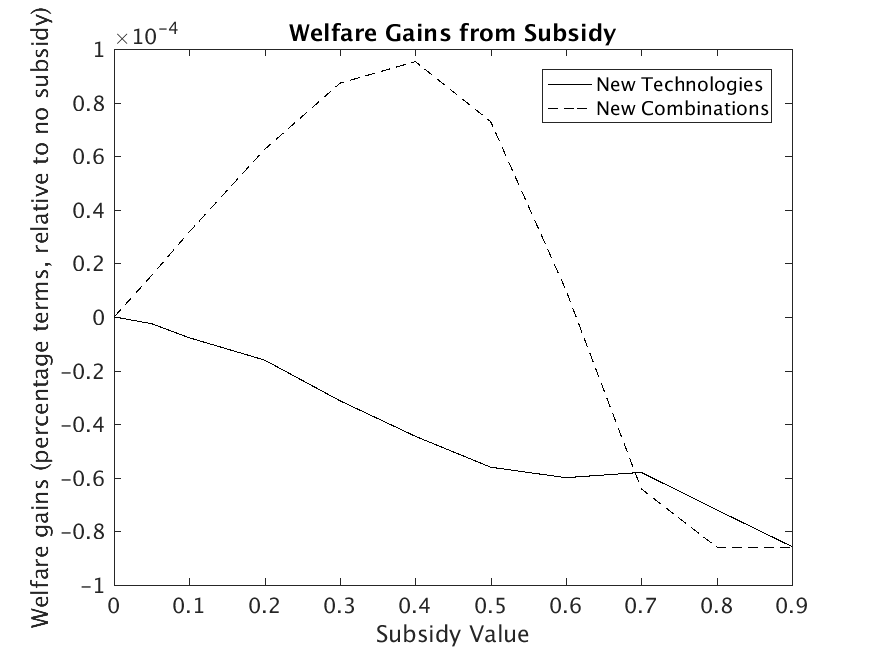
\includegraphics[width=.7\textwidth]{figures/2_years/welfare_gains.png}
\caption{Welfare gains after a subsidy that lasts 2 years.}
\end{figure}

\clearpage

\begin{figure}[h!]
\centering
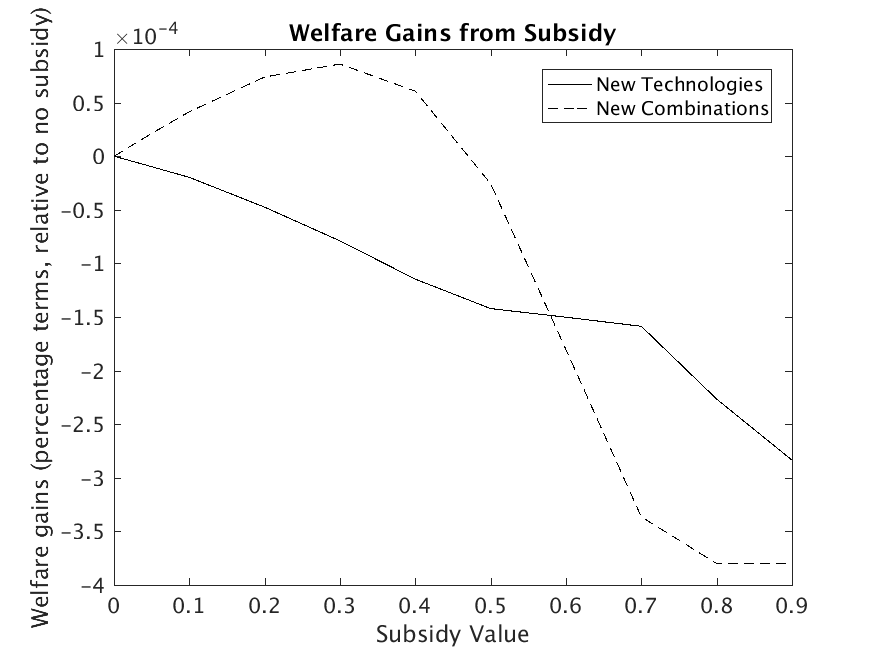
\includegraphics[width=.7\textwidth]{figures/5_years/welfare_gains.png}
\caption{Welfare gains after a subsidy that lasts 5 years.}
\end{figure}

\begin{figure}[h!]
\centering
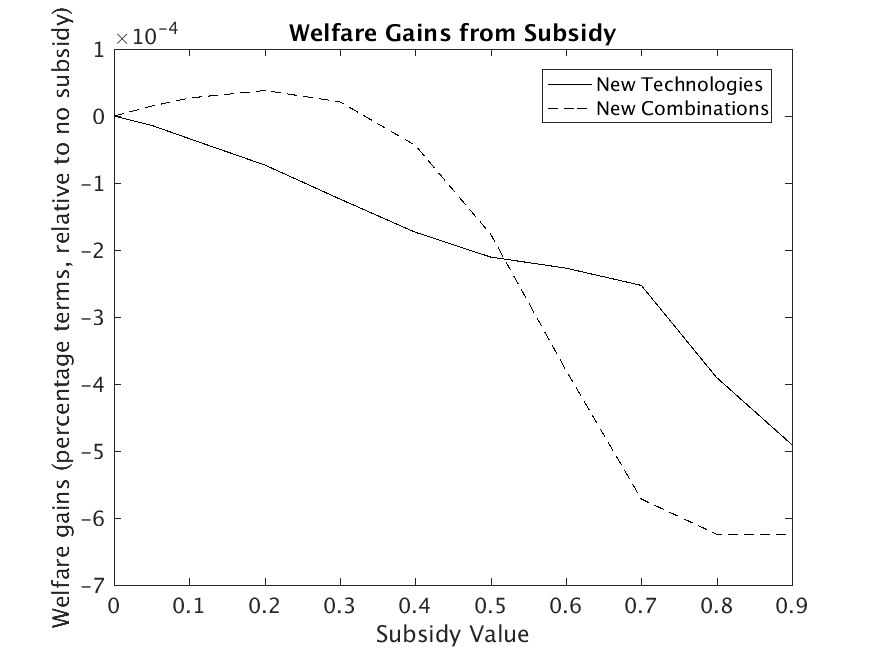
\includegraphics[width=.7\textwidth]{figures/7_years/welfare_gains.png}
\caption{Welfare gains after a subsidy that lasts 7 years.}
\end{figure}

\clearpage

\begin{figure}[h!]
\centering
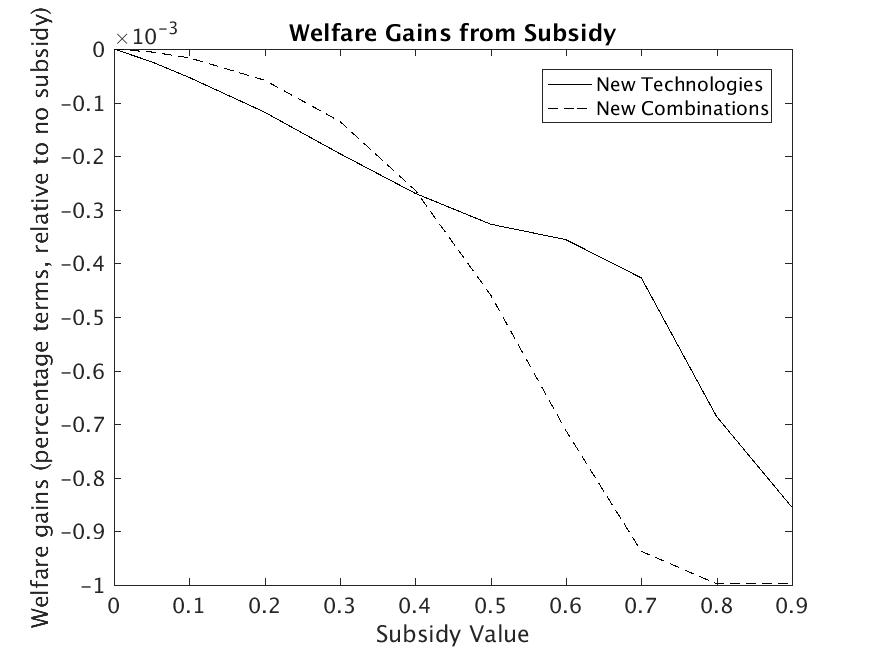
\includegraphics[width=.7\textwidth]{figures/10_years/welfare_gains.png}
\caption{Welfare gains after a subsidy that lasts 10 years.}
\end{figure}

\section{Summary of the Economy}

In what follows, I present a brief description of the main variables in the economy. This includes both the evolution of the economy without subsidy (from 1836 to 2016) and the economy with subsidy (2017 to 2027). For the economy with subsidy, I chose to show what happens to those variables when a 50\% subsidy is implemented for 5 years. Note, however, that all of the plots extend for 10 years after the initial date, even though the subsidy only lasts for 5.

\subsection{Evolution of Economy without subsidy}

\begin{figure}[h!]
\begin{subfigure}[b]{0.45\textwidth}
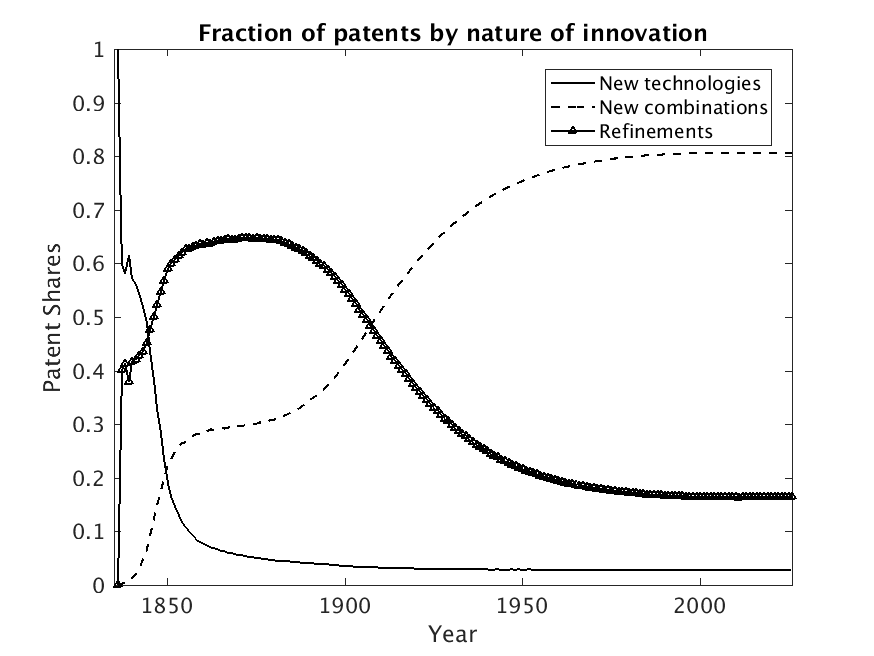
\includegraphics[width=\textwidth]{figures/5_years/patents.png}
\subcaption{Model.}
\end{subfigure}
\begin{subfigure}[b]{0.45\textwidth}
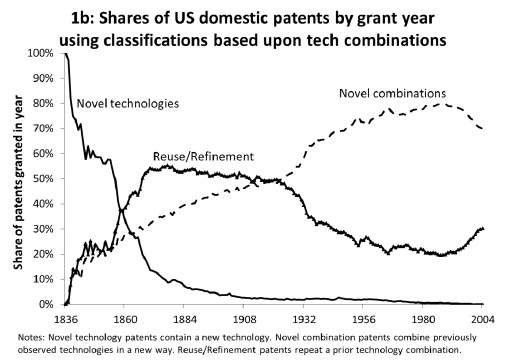
\includegraphics[width=\textwidth]{figures/patents_data.png}
\subcaption{Data.}
\end{subfigure}
\end{figure}

\begin{figure}[h!]
\centering
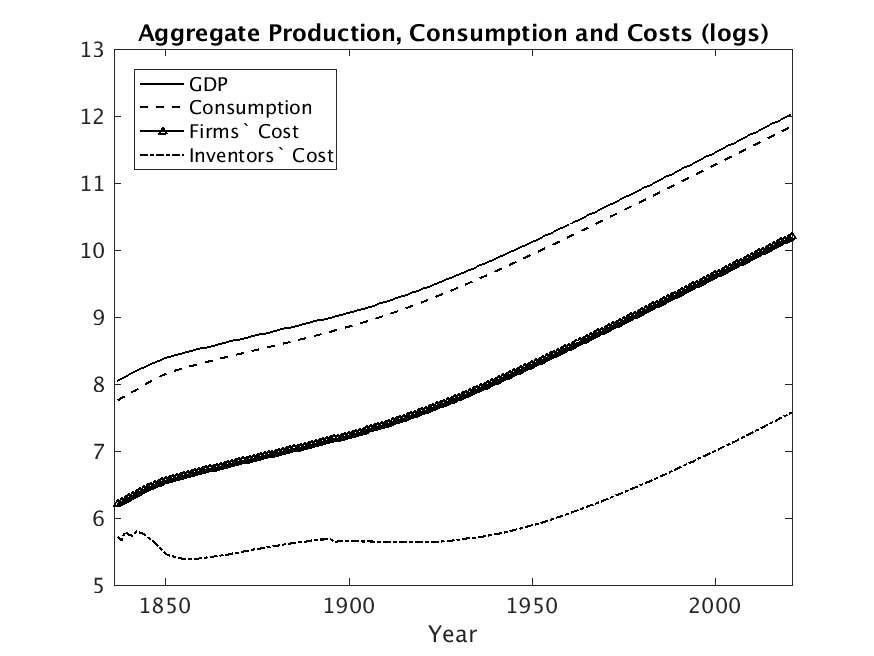
\includegraphics[width=.7\textwidth]{figures/5_years/aggregates.png}
\caption{Value of aggregate variables in the economy.}
\end{figure}

\begin{figure}[h!]
\centering
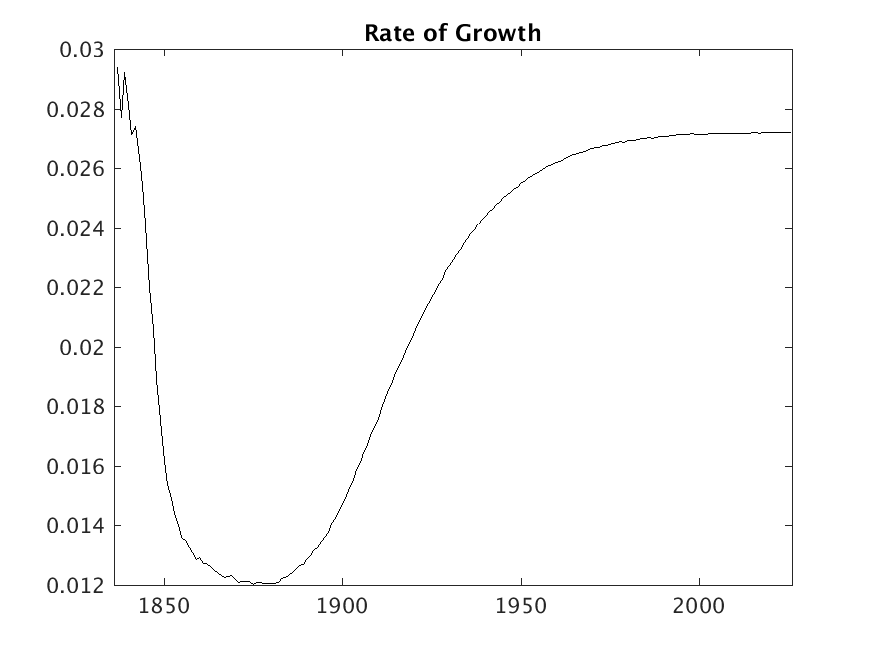
\includegraphics[width=.7\textwidth]{figures/5_years/growth.png}
\caption{Evolution of the rate of growth.}
\end{figure}

\begin{figure}[h!]
\centering
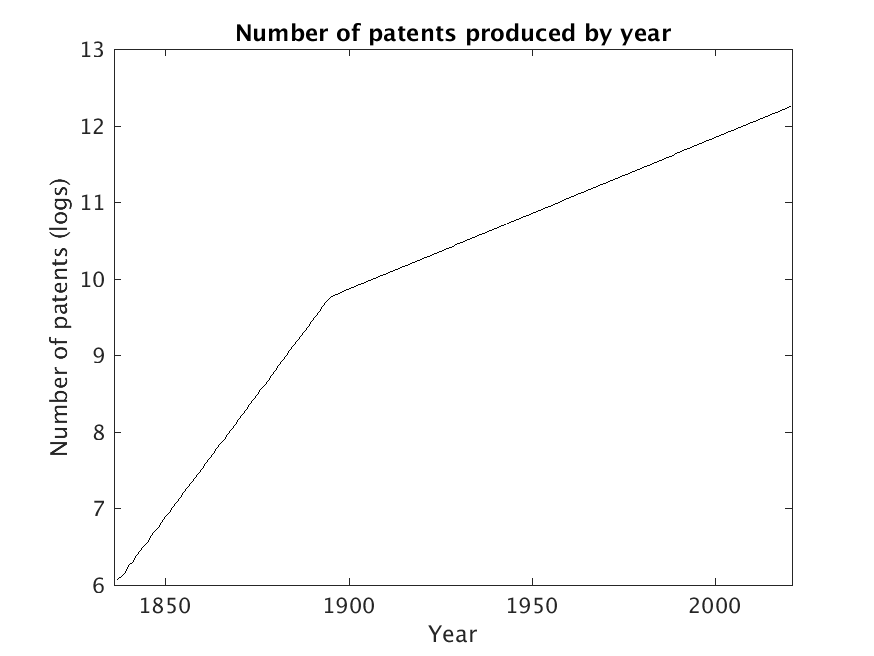
\includegraphics[width=.7\textwidth]{figures/5_years/num_pats.png}
\caption{Number of patents produced each period.}
\end{figure}

\clearpage

\subsection*{Economy with Subsidy}

\begin{figure}[h!]
\centering
\includegraphics[width=.7\textwidth]{figures/5_years/gdp_subs.png}
\caption{Change in GDP after subsidies.}
\end{figure}

\begin{figure}[h!]
\centering
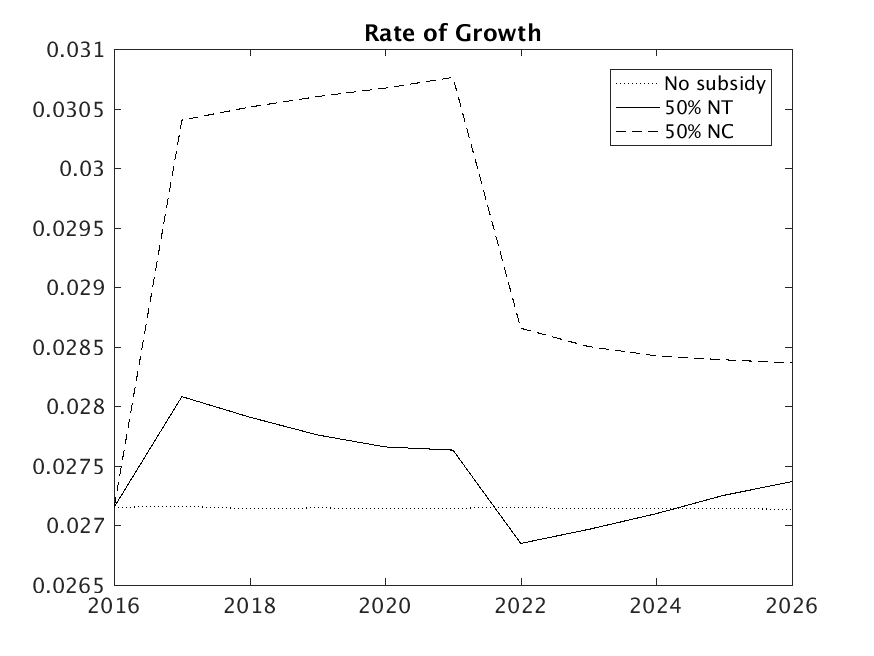
\includegraphics[width=.7\textwidth]{figures/5_years/growth_subs.png}
\caption{Change in growth rate after subsidies.}
\end{figure}

\begin{figure}[h!]
\centering
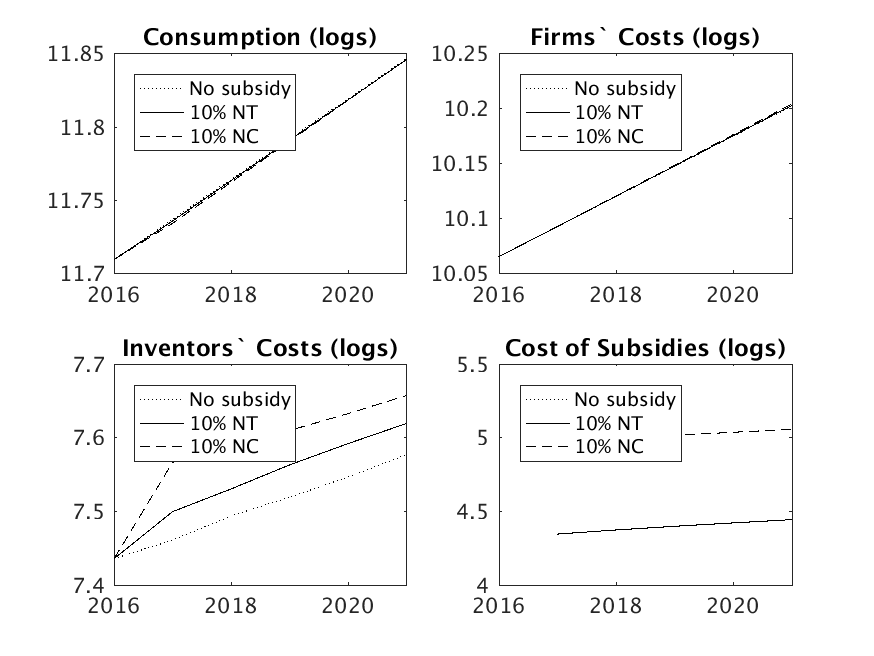
\includegraphics[width=\textwidth]{figures/5_years/aggregates_subs.png}
\caption{Change in aggregates after subsidies.}
\end{figure}


\begin{figure}[h!]
\centering
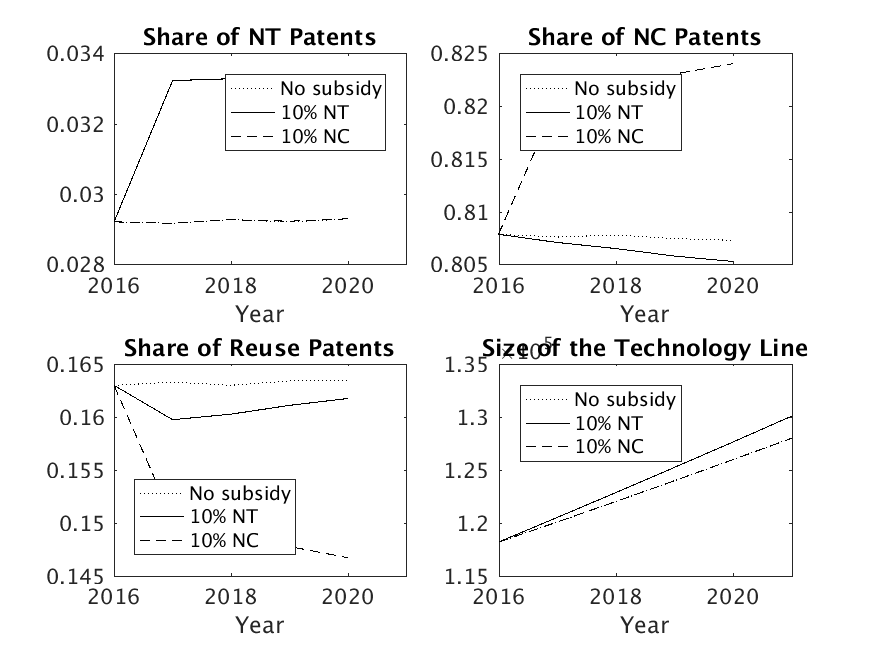
\includegraphics[width=\textwidth]{figures/5_years/patent_subs.png}
\caption{Change in patent shares after subsidies.}
\end{figure}


\end{document}


%#############################################


\begin{itemize}
\item The value of the subsidies considered were: 2, 5, 10, 20 and 30\% for both new technologies or new combinations. We could do more, but the simulations tend to take longer when subsidies are higher.
\item The subsidy runs for 30 years, starting in 2016 (180 years after the simulations starts).
\item I ran 20 simulations of the model. 
\end{itemize}

\begin{figure}[h!]
\begin{subfigure}[b]{0.45\textwidth}
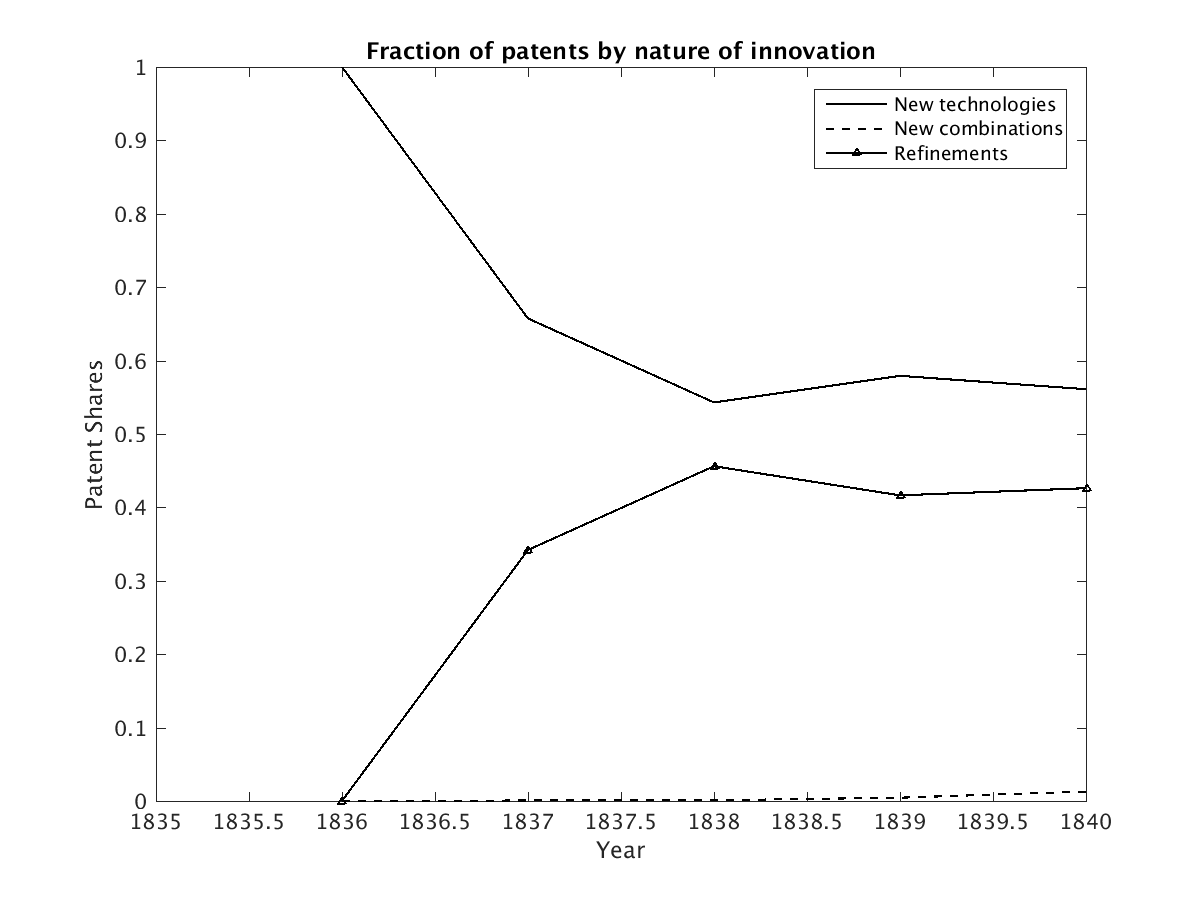
\includegraphics[width=\textwidth]{figures/patents.png}
\subcaption{Model.}
\end{subfigure}
\begin{subfigure}[b]{0.45\textwidth}
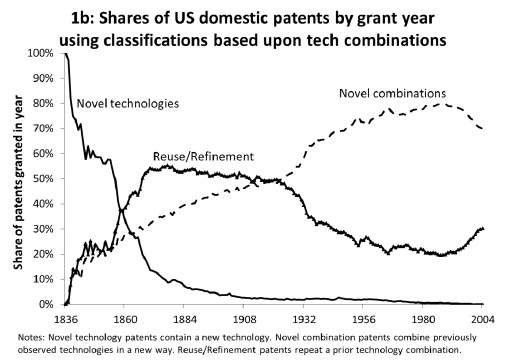
\includegraphics[width=\textwidth]{figures/patents_data.png}
\subcaption{Data.}
\end{subfigure}
\end{figure}

\begin{figure}[h!]
\centering
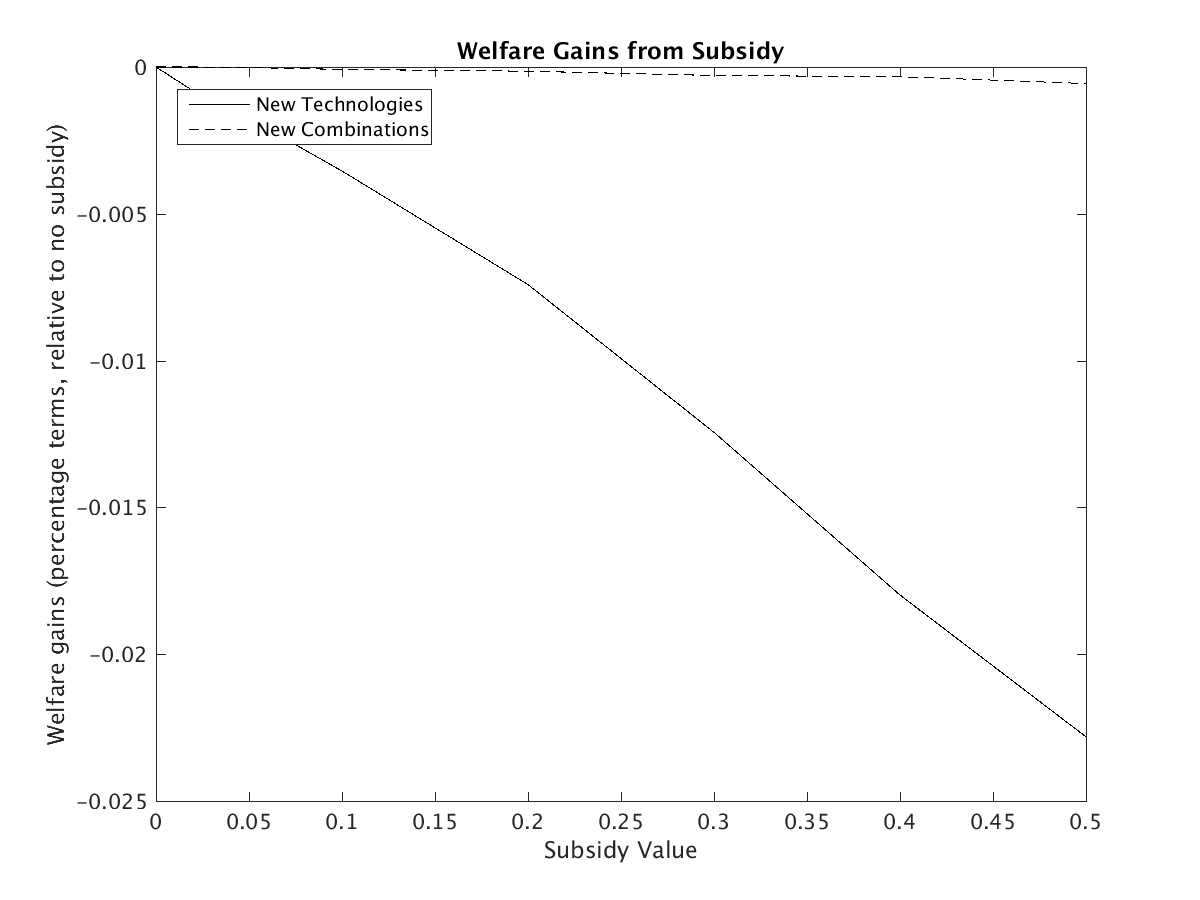
\includegraphics[width=.8\textwidth]{figures/welfare_gains.png}
\end{figure}

\clearpage

\section*{Other Figures}

\subsection*{Evolution of Economy without subsidy}

\begin{figure}[h!]
\centering
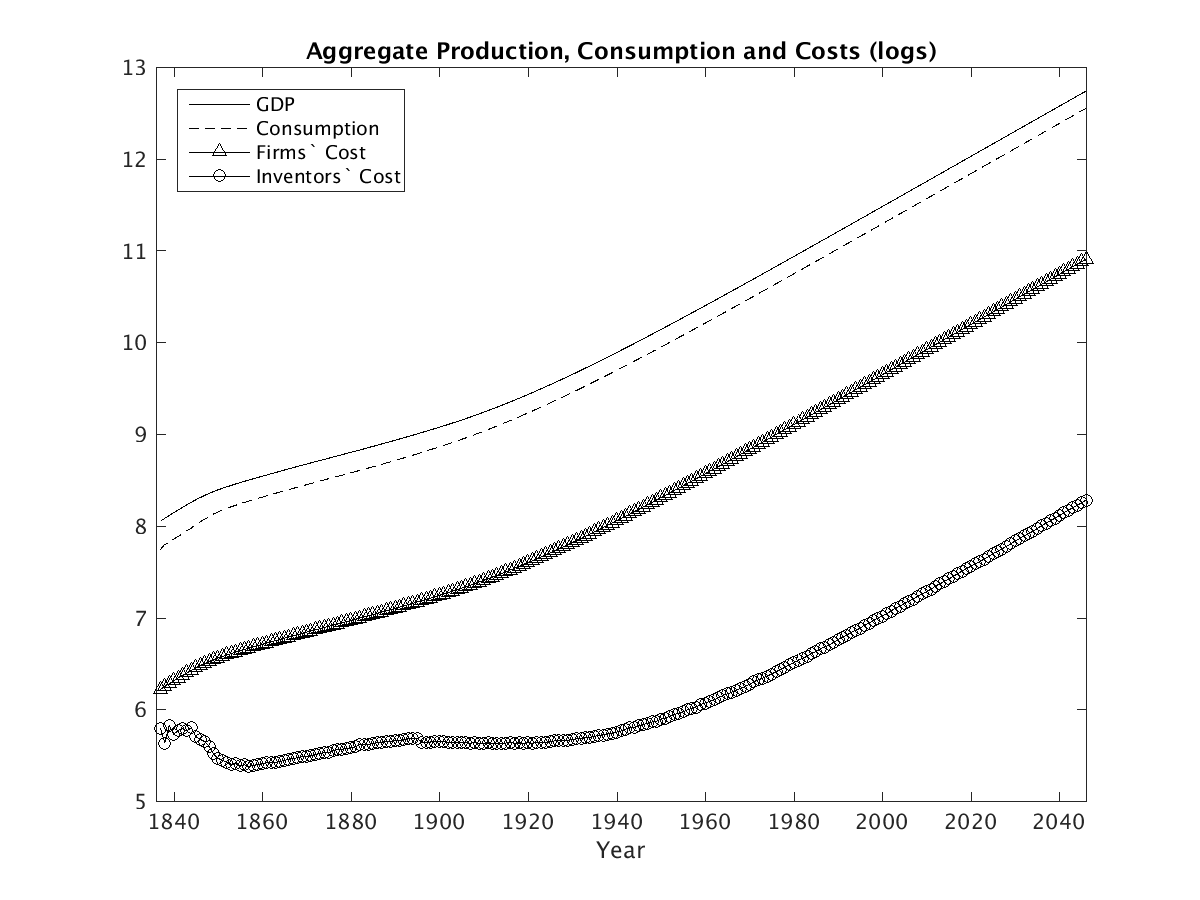
\includegraphics[width=\textwidth]{figures/aggregates.png}
\caption{Value of aggregate variables in the economy.}
\end{figure}

\begin{figure}[h!]
\centering
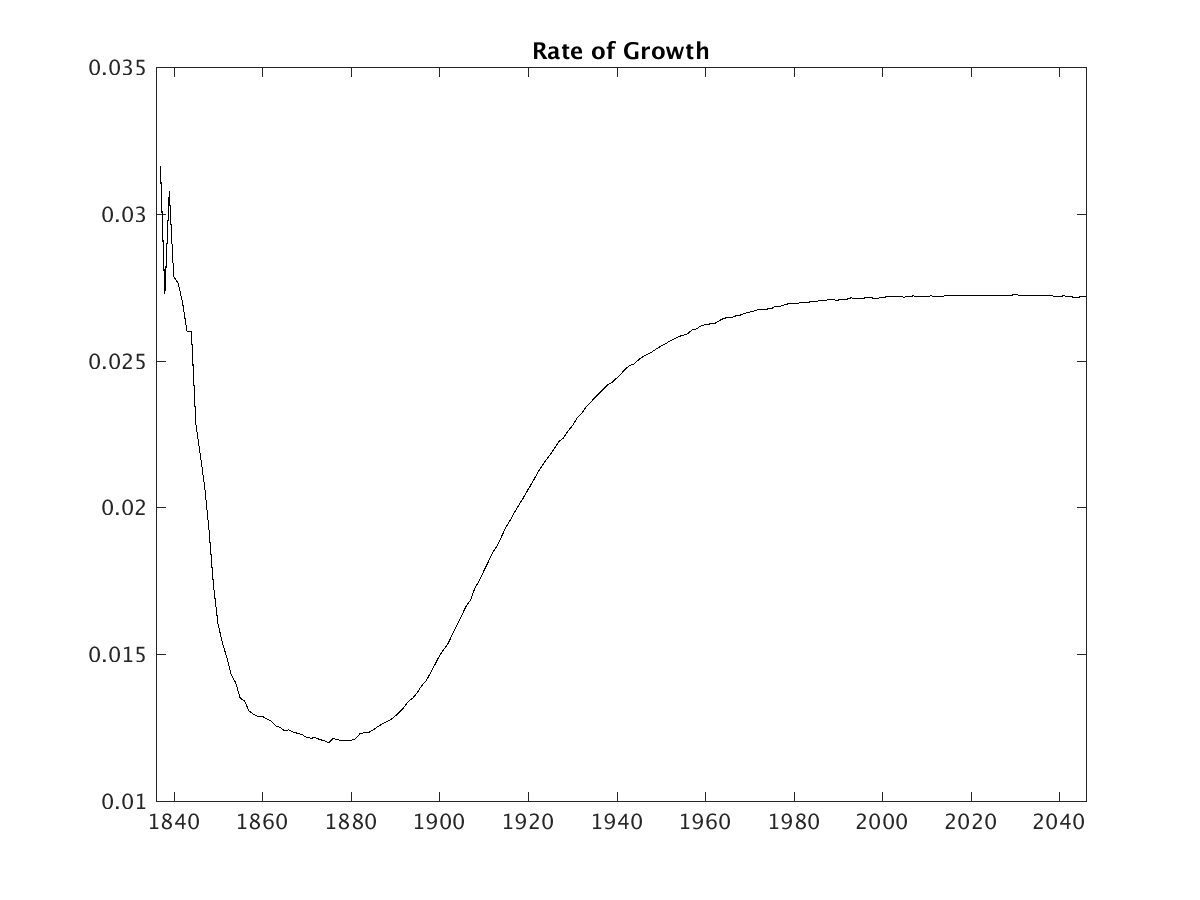
\includegraphics[width=.75\textwidth]{figures/growth.png}
\caption{Evolution of the rate of growth.}
\end{figure}

\begin{figure}[h!]
\centering
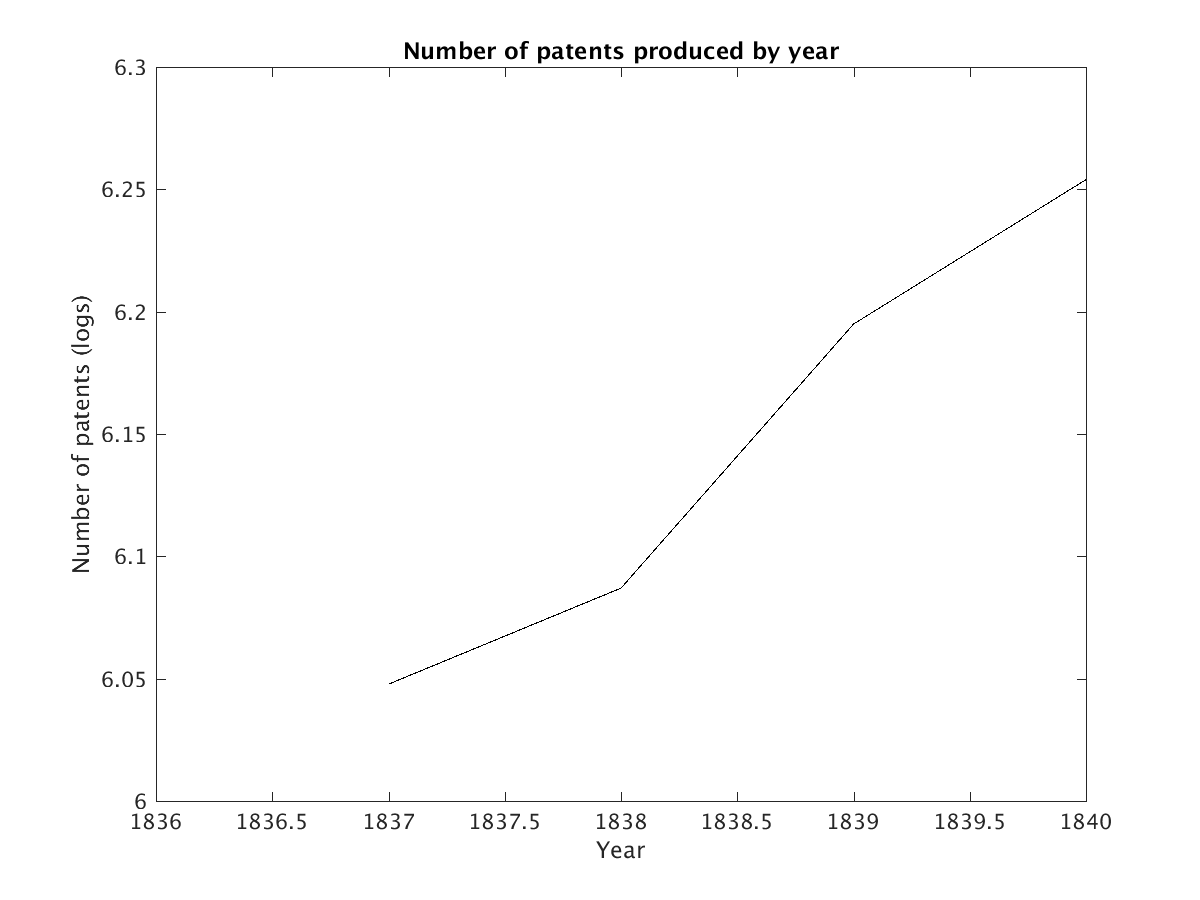
\includegraphics[width=.75\textwidth]{figures/num_pats.png}
\caption{Number of patents produced each period.}
\end{figure}

\clearpage

\subsection*{Economy with a 10\% Subsidy}

\begin{figure}[h!]
\centering
\includegraphics[width=\textwidth]{figures/gdp_subs.png}
\caption{Change in GDP after subsidies.}
\end{figure}

\begin{figure}[h!]
\centering
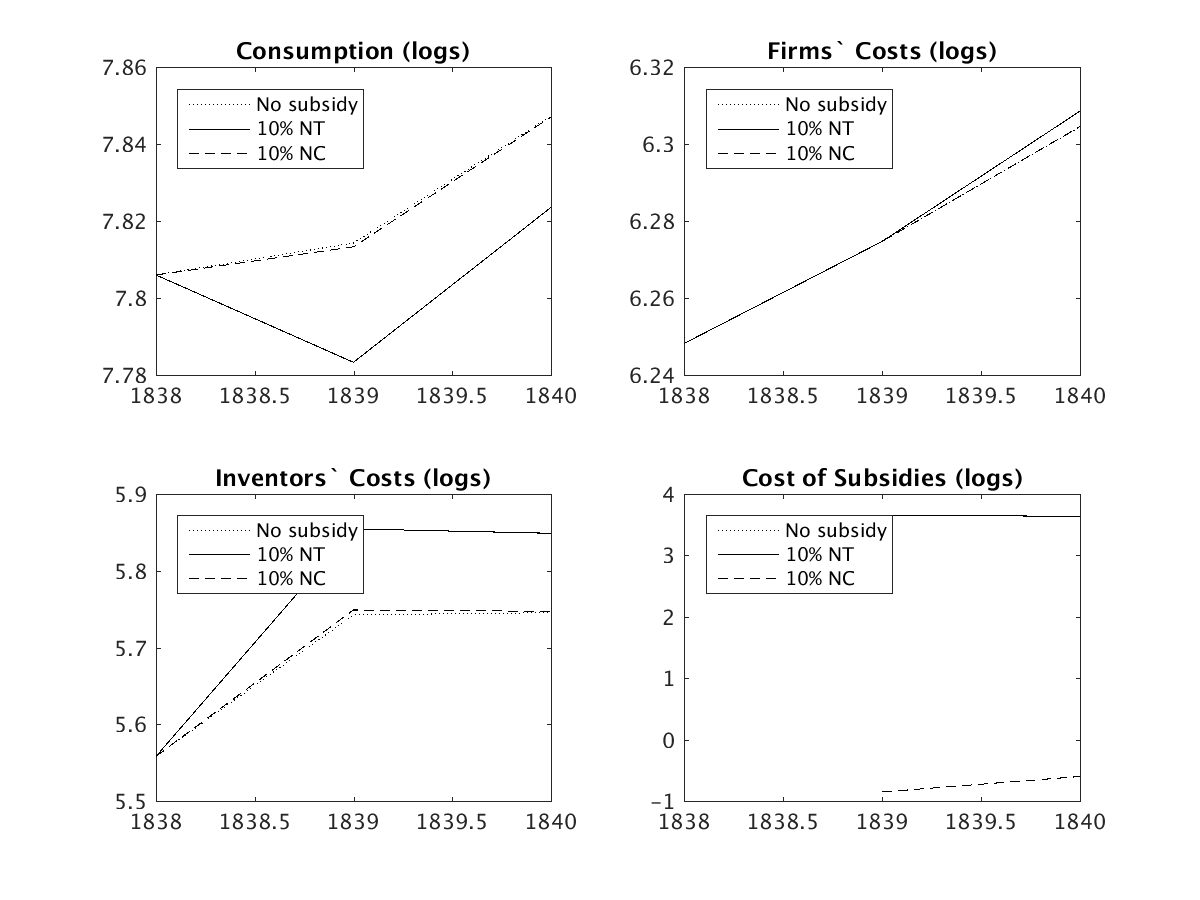
\includegraphics[width=\textwidth]{figures/aggregates_subs.png}
\caption{Change in aggregates after subsidies.}
\end{figure}

\begin{figure}[h!]
\centering
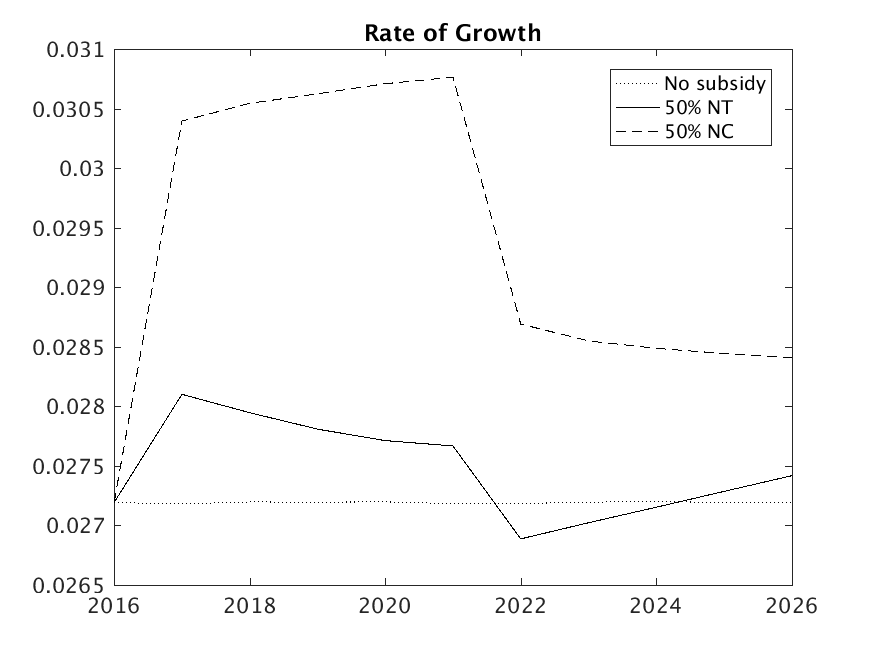
\includegraphics[width=\textwidth]{figures/growth_subs.png}
\caption{Change in growth rate after subsidies.}
\end{figure}

\begin{figure}[h!]
\centering
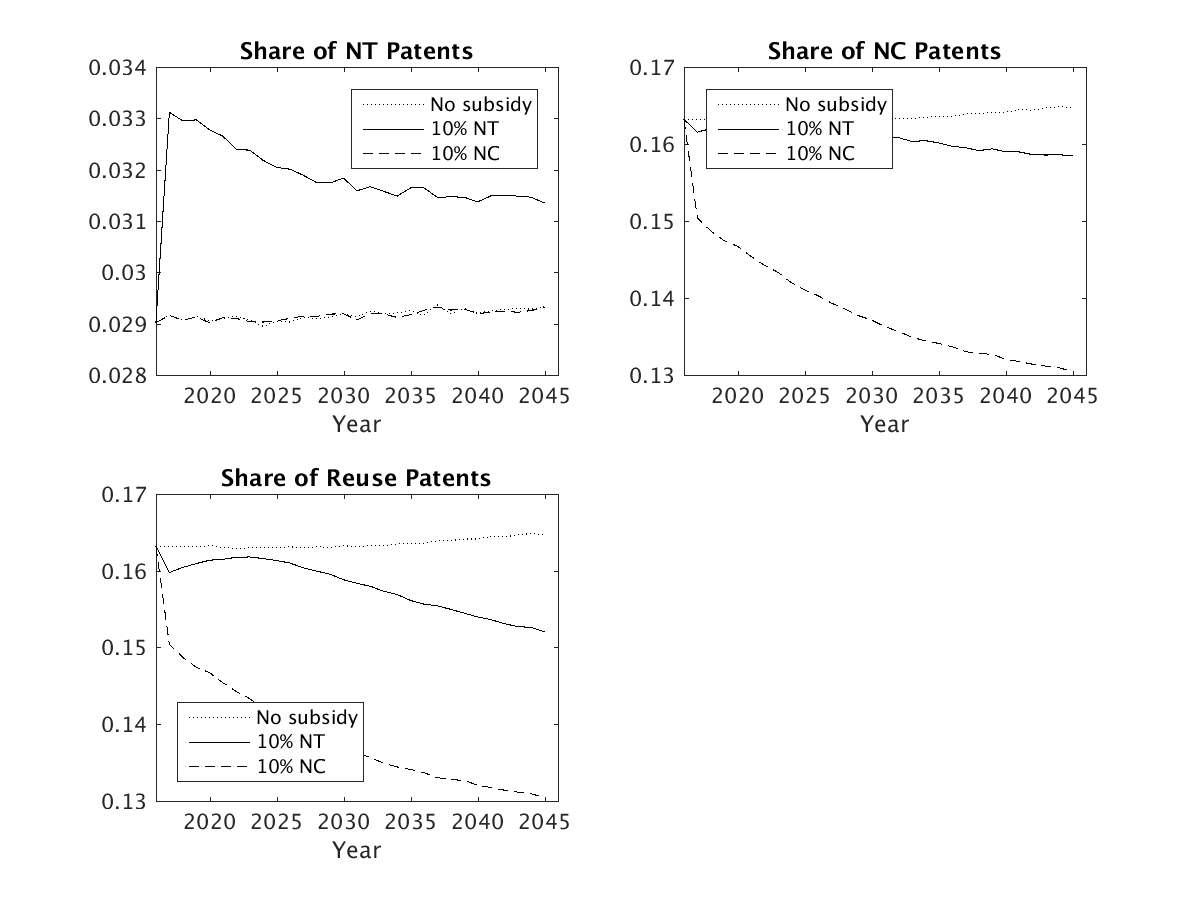
\includegraphics[width=\textwidth]{figures/patent_subs.png}
\caption{Change in patent shares after subsidies.}
\end{figure}







\end{document}